\input{header.tex}
\input{newcommands.tex}

\title{Venn-Diagramme mit Ti\textit{k}Z in \hologo{LaTeX}}
\author{Fortbildungsmaterial für MINT-Lehrkräfte}
\date{13. Mai 2025}
\pagestyle{plain}


\begin{document}

\maketitle

TikZ bietet mit der \texttt{intersections}-Bibliothek leistungsfähige Möglichkeiten zur Darstellung von Venn-Diagrammen in der Mengenlehre. Diese Handreichung führt Sie in die Techniken des Zeichnens von Mengendiagrammen ein und zeigt, wie Sie typische Mengenoperationen wie Vereinigung, Durchschnitt, Differenz und Komplement visualisieren können.

\section{Grundlagen: Zwei Mengen zeichnen}

Um Venn-Diagramme zu erstellen, benötigen wir zunächst die \texttt{intersections}-Bibliothek:

\begin{lstlisting}[style=latex]
\usepackage{tikz}
\usetikzlibrary{intersections, patterns, calc}
\end{lstlisting}

Die Grundidee besteht darin, Kreise mit benannten Pfaden zu definieren und dann mit dem \texttt{clip}-Befehl die gewünschten Bereiche zu füllen. Beginnen wir mit zwei einfachen Mengen:

\begin{lstlisting}[style=latex]
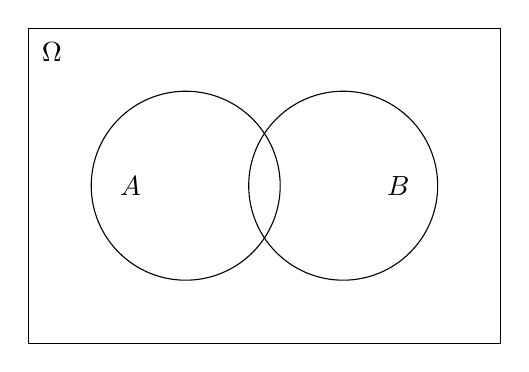
\begin{tikzpicture}
    % Rechteck fuer die Grundmenge zeichnen
    \draw (0,0) rectangle (6,4);
    
    % Menge A (linker Kreis)
    \draw (2,2) circle (1.2cm);
    \node at (1.3,2) {$A$};
    
    % Menge B (rechter Kreis)
    \draw (4,2) circle (1.2cm);
    \node at (4.7,2) {$B$};
    
    % Beschriftung der Grundmenge
    \node at (0.3,3.7) {$\Omega$};
\end{tikzpicture}
\end{lstlisting}

\begin{ausgabe}

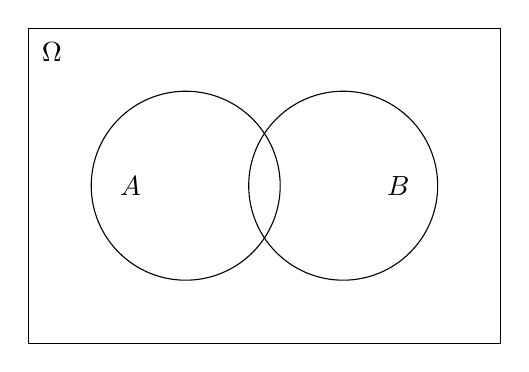
\begin{tikzpicture}
    \draw (0,0) rectangle (6,4);
    \draw (2,2) circle (1.2cm);
    \node at (1.3,2) {$A$};
    \draw (4,2) circle (1.2cm);
    \node at (4.7,2) {$B$};
    \node at (0.3,3.7) {$\Omega$};
\end{tikzpicture}
\end{ausgabe}

\section{Mengenoperationen mit \texttt{scope} und \texttt{clip}}

Um verschiedene Mengenbereiche zu färben, nutzen wir die \texttt{scope}-Umgebung in Kombination mit \texttt{clip}. Der Trick besteht darin, durch geschicktes Clipping die gewünschten Bereiche zu isolieren.

\subsection{Die Menge $A$ füllen}

\begin{lstlisting}[style=latex]
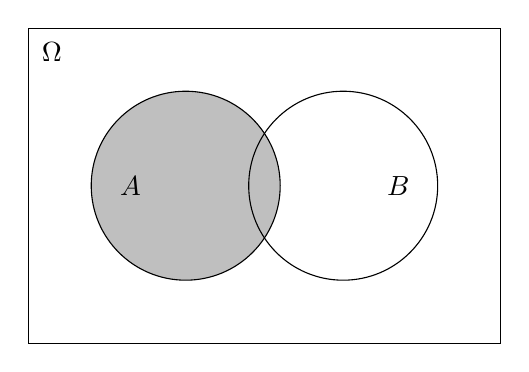
\begin{tikzpicture}
    % Menge A fuellen
    \begin{scope}
        \fill[gray, opacity=0.5] (2,2) circle (1.2cm);
    \end{scope}
    
    % Konturen zeichnen
    \draw (0,0) rectangle (6,4);
    \draw (2,2) circle (1.2cm);
    \draw (4,2) circle (1.2cm);
    \node at (1.3,2) {$A$};
    \node at (4.7,2) {$B$};
    \node at (0.3,3.7) {$\Omega$};
\end{tikzpicture}
\end{lstlisting}

\begin{ausgabe}
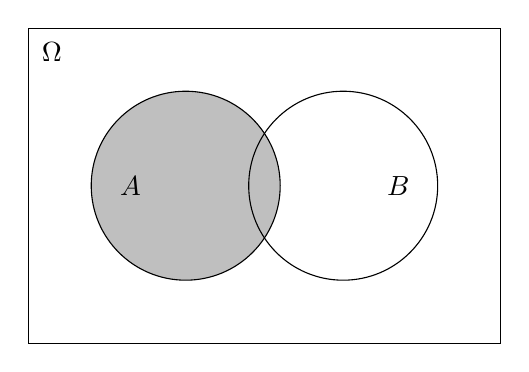
\begin{tikzpicture}
    \begin{scope}
        \fill[gray, opacity=0.5] (2,2) circle (1.2cm);
    \end{scope}
    \draw (0,0) rectangle (6,4);
    \draw (2,2) circle (1.2cm);
    \draw (4,2) circle (1.2cm);
    \node at (1.3,2) {$A$};
    \node at (4.7,2) {$B$};
    \node at (0.3,3.7) {$\Omega$};
\end{tikzpicture}
\end{ausgabe}

\subsection{Die Vereinigung $A \cup B$ füllen}

\begin{lstlisting}[style=latex]
% Vereinigung von A und B mit intersections
\begin{tikzpicture}
    % Kreise mit Namen definieren
    \path[name path=A] (2,2) circle (1.2cm);
    \path[name path=B] (4,2) circle (1.2cm);
    
    % Beide Mengen fuellen
    \fill[gray, opacity=0.5, name path=A] (2,2) circle (1.2cm);
    \fill[gray, opacity=0.5, name path=B] (4,2) circle (1.2cm);
    
    \draw (0,0) rectangle (6,4);
    \draw (2,2) circle (1.2cm);
    \draw (4,2) circle (1.2cm);
    \node at (1.3,2) {$A$};
    \node at (4.7,2) {$B$};
    \node at (0.3,3.7) {$\Omega$};
\end{tikzpicture}
\end{lstlisting}

\begin{ausgabe}
\begin{tikzpicture}
    % Kreise mit Namen definieren
    \path[name path=A] (2,2) circle (1.2cm);
    \path[name path=B] (4,2) circle (1.2cm);
    
    % Beide Mengen fuellen
    \fill[gray, opacity=0.5, name path=A] (2,2) circle (1.2cm);
    \fill[gray, opacity=0.5, name path=B] (4,2) circle (1.2cm);
    
    \draw (0,0) rectangle (6,4);
    \draw (2,2) circle (1.2cm);
    \draw (4,2) circle (1.2cm);
    \node at (1.3,2) {$A$};
    \node at (4.7,2) {$B$};
    \node at (0.3,3.7) {$\Omega$};
\end{tikzpicture}
\end{ausgabe}

\subsection{Den Durchschnitt $A \cap B$ füllen}

Der Durchschnitt wird durch Clipping auf beide Kreise realisiert:

\begin{lstlisting}[style=latex]
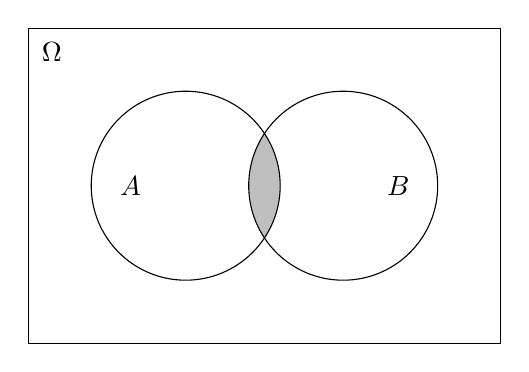
\begin{tikzpicture}
    % Durchschnitt von A und B fuellen
    \begin{scope}
        \clip (2,2) circle (1.2cm);
        \fill[gray, opacity=0.5] (4,2) circle (1.2cm);
    \end{scope}
    
    \draw (0,0) rectangle (6,4);
    \draw (2,2) circle (1.2cm);
    \draw (4,2) circle (1.2cm);
    \node at (1.3,2) {$A$};
    \node at (4.7,2) {$B$};
    \node at (0.3,3.7) {$\Omega$};
\end{tikzpicture}
\end{lstlisting}

\begin{ausgabe}
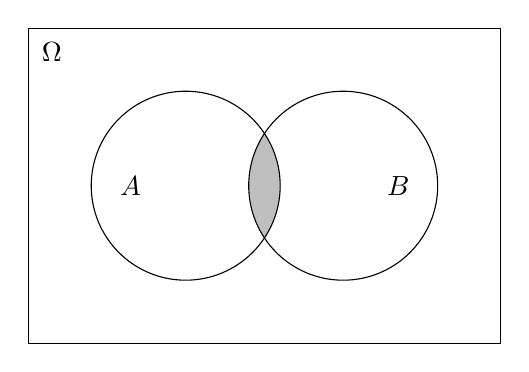
\begin{tikzpicture}
    \begin{scope}
        \clip (2,2) circle (1.2cm);
        \fill[gray, opacity=0.5] (4,2) circle (1.2cm);
    \end{scope}
    \draw (0,0) rectangle (6,4);
    \draw (2,2) circle (1.2cm);
    \draw (4,2) circle (1.2cm);
    \node at (1.3,2) {$A$};
    \node at (4.7,2) {$B$};
    \node at (0.3,3.7) {$\Omega$};
\end{tikzpicture}
\end{ausgabe}

Die \texttt{clip}-Anweisung beschränkt alle nachfolgenden Zeichenoperationen auf den angegebenen Bereich. Durch \texttt{\textbackslash clip (2,2) circle (1.2cm)} wird zunächst auf den Bereich von Menge $A$ eingeschränkt. Anschließend wird Menge $B$ gefüllt, wobei nur der Teil innerhalb von $A$ sichtbar wird – genau der Durchschnitt $A \cap B$.

\subsection{Die Differenz $A \setminus B$ füllen}

Die Differenz $A \setminus B$ (alle Elemente, die in $A$, aber nicht in $B$ liegen) wird durch geschicktes Clipping realisiert:

\begin{lstlisting}[style=latex]
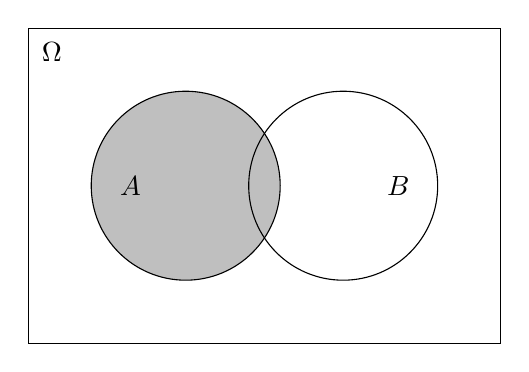
\begin{tikzpicture}
    % Differenz von A und B fuellen
    \begin{scope}
        \clip (2,2) circle (1.2cm);
        \fill[white] (4,2) circle (1.2cm);
        \fill[gray, opacity=0.5] (2,2) circle (1.2cm);
    \end{scope}
    
    \draw (0,0) rectangle (6,4);
    \draw (2,2) circle (1.2cm);
    \draw (4,2) circle (1.2cm);
    \node at (1.3,2) {$A$};
    \node at (4.7,2) {$B$};
    \node at (0.3,3.7) {$\Omega$};
\end{tikzpicture}
\end{lstlisting}

\begin{ausgabe}
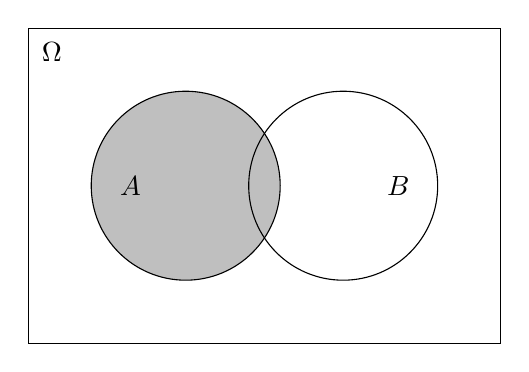
\begin{tikzpicture}
    \begin{scope}
        \clip (2,2) circle (1.2cm);
        \fill[white] (4,2) circle (1.2cm);
        \fill[gray, opacity=0.5] (2,2) circle (1.2cm);
    \end{scope}
    \draw (0,0) rectangle (6,4);
    \draw (2,2) circle (1.2cm);
    \draw (4,2) circle (1.2cm);
    \node at (1.3,2) {$A$};
    \node at (4.7,2) {$B$};
    \node at (0.3,3.7) {$\Omega$};
\end{tikzpicture}
\end{ausgabe}

Hier wird zunächst auf Menge $A$ geclippt, dann der Bereich von $B$ weiß gefüllt (um ihn auszusparen) und schließlich $A$ gefärbt. Das Ergebnis zeigt nur den Teil von $A$, der nicht zu $B$ gehört.

\subsection{Die symmetrische Differenz $A \triangle B$ füllen}

Die symmetrische Differenz $(A \setminus B) \cup (B \setminus A)$ enthält alle Elemente, die entweder in $A$ oder in $B$, aber nicht in beiden liegen:

\begin{lstlisting}[style=latex]
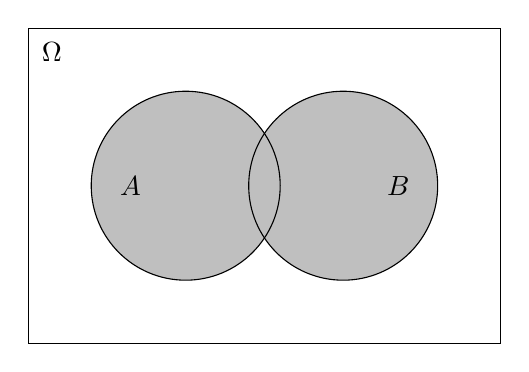
\begin{tikzpicture}
    % Symmetrische Differenz von A und B fuellen
    \begin{scope}
        \clip (2,2) circle (1.2cm);
        \fill[white] (4,2) circle (1.2cm);
        \fill[gray, opacity=0.5] (2,2) circle (1.2cm);
    \end{scope}
    \begin{scope}
        \clip (4,2) circle (1.2cm);
        \fill[white] (2,2) circle (1.2cm);
        \fill[gray, opacity=0.5] (4,2) circle (1.2cm);
    \end{scope}
    
    \draw (0,0) rectangle (6,4);
    \draw (2,2) circle (1.2cm);
    \draw (4,2) circle (1.2cm);
    \node at (1.3,2) {$A$};
    \node at (4.7,2) {$B$};
    \node at (0.3,3.7) {$\Omega$};
\end{tikzpicture}
\end{lstlisting}

\begin{ausgabe}
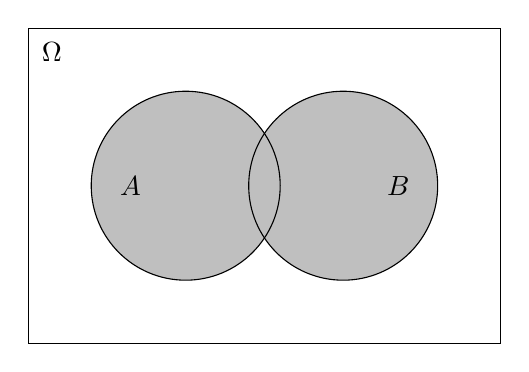
\begin{tikzpicture}
    \begin{scope}
        \clip (2,2) circle (1.2cm);
        \fill[white] (4,2) circle (1.2cm);
        \fill[gray, opacity=0.5] (2,2) circle (1.2cm);
    \end{scope}
    \begin{scope}
        \clip (4,2) circle (1.2cm);
        \fill[white] (2,2) circle (1.2cm);
        \fill[gray, opacity=0.5] (4,2) circle (1.2cm);
    \end{scope}
    \draw (0,0) rectangle (6,4);
    \draw (2,2) circle (1.2cm);
    \draw (4,2) circle (1.2cm);
    \node at (1.3,2) {$A$};
    \node at (4.7,2) {$B$};
    \node at (0.3,3.7) {$\Omega$};
\end{tikzpicture}
\end{ausgabe}

\subsection{Das Komplement $\overline{A}$ füllen}

Das Komplement von $A$ umfasst alle Elemente der Grundmenge, die nicht in $A$ liegen:

\begin{lstlisting}[style=latex]
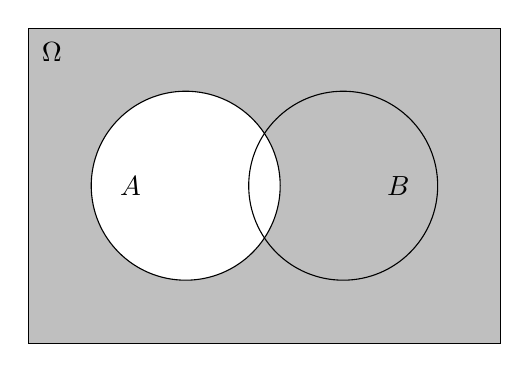
\begin{tikzpicture}
    % Komplement von A fuellen
    \begin{scope}
        \clip (0,0) rectangle (6,4);
        \fill[gray, opacity=0.5] (0,0) rectangle (6,4);
        \fill[white] (2,2) circle (1.2cm);
    \end{scope}
    
    \draw (0,0) rectangle (6,4);
    \draw (2,2) circle (1.2cm);
    \draw (4,2) circle (1.2cm);
    \node at (1.3,2) {$A$};
    \node at (4.7,2) {$B$};
    \node at (0.3,3.7) {$\Omega$};
\end{tikzpicture}
\end{lstlisting}

\begin{ausgabe}
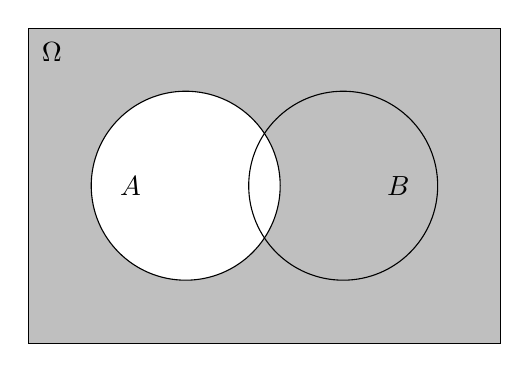
\begin{tikzpicture}
    \begin{scope}
        \clip (0,0) rectangle (6,4);
        \fill[gray, opacity=0.5] (0,0) rectangle (6,4);
        \fill[white] (2,2) circle (1.2cm);
    \end{scope}
    \draw (0,0) rectangle (6,4);
    \draw (2,2) circle (1.2cm);
    \draw (4,2) circle (1.2cm);
    \node at (1.3,2) {$A$};
    \node at (4.7,2) {$B$};
    \node at (0.3,3.7) {$\Omega$};
\end{tikzpicture}
\end{ausgabe}

\section{Drei Mengen zeichnen}

Bei drei Mengen wird es interessanter, da sich mehr Schnittbereiche ergeben. Die Grundstruktur bleibt jedoch die gleiche:

\begin{lstlisting}[style=latex]
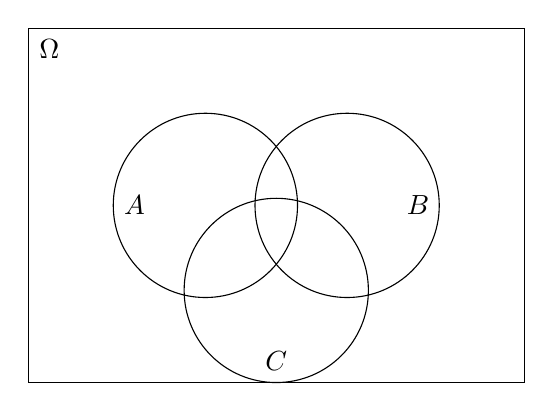
\begin{tikzpicture}[scale=0.9]
    % Rechteck fuer die Grundmenge
    \draw (0,0) rectangle (7,5);
    
    % Menge A (linker Kreis)
    \draw (2.5,2.5) circle (1.3cm);
    \node at (1.5,2.5) {$A$};
    
    % Menge B (rechter Kreis)
    \draw (4.5,2.5) circle (1.3cm);
    \node at (5.5,2.5) {$B$};
    
    % Menge C (unterer Kreis)
    \draw (3.5,1.3) circle (1.3cm);
    \node at (3.5,0.3) {$C$};
    
    % Beschriftung der Grundmenge
    \node at (0.3,4.7) {$\Omega$};
\end{tikzpicture}
\end{lstlisting}

\begin{ausgabe}
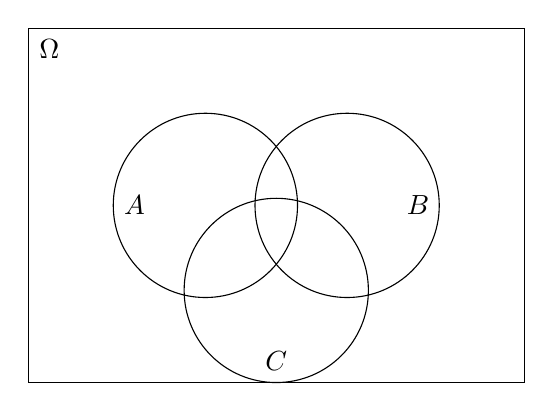
\begin{tikzpicture}[scale=0.9]
    \draw (0,0) rectangle (7,5);
    \draw (2.5,2.5) circle (1.3cm);
    \node at (1.5,2.5) {$A$};
    \draw (4.5,2.5) circle (1.3cm);
    \node at (5.5,2.5) {$B$};
    \draw (3.5,1.3) circle (1.3cm);
    \node at (3.5,0.3) {$C$};
    \node at (0.3,4.7) {$\Omega$};
\end{tikzpicture}
\end{ausgabe}

\subsection{Den Durchschnitt $A \cap B \cap C$ füllen}

Der Durchschnitt aller drei Mengen wird durch dreifaches Clipping erreicht:

\begin{lstlisting}[style=latex]
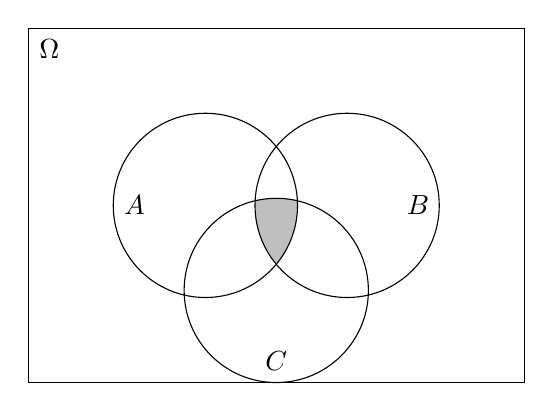
\begin{tikzpicture}[scale=0.9]
    % Durchschnitt von A und  B und C fuellen
    \begin{scope}
        \clip (2.5,2.5) circle (1.3cm);
        \clip (4.5,2.5) circle (1.3cm);
        \fill[gray, opacity=0.5] (3.5,1.3) circle (1.3cm);
    \end{scope}
    
    \draw (0,0) rectangle (7,5);
    \draw (2.5,2.5) circle (1.3cm);
    \draw (4.5,2.5) circle (1.3cm);
    \draw (3.5,1.3) circle (1.3cm);
    \node at (1.5,2.5) {$A$};
    \node at (5.5,2.5) {$B$};
    \node at (3.5,0.3) {$C$};
    \node at (0.3,4.7) {$\Omega$};
\end{tikzpicture}
\end{lstlisting}

\begin{ausgabe}
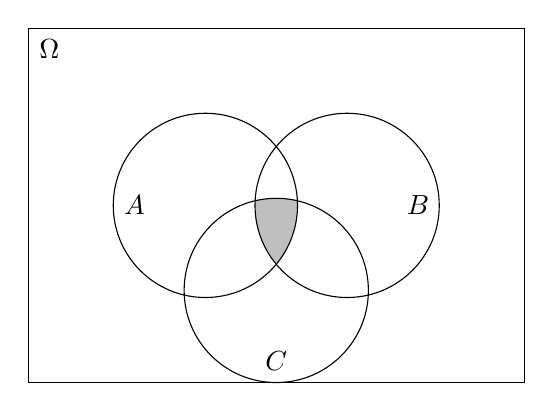
\begin{tikzpicture}[scale=0.9]
    \begin{scope}
        \clip (2.5,2.5) circle (1.3cm);
        \clip (4.5,2.5) circle (1.3cm);
        \fill[gray, opacity=0.5] (3.5,1.3) circle (1.3cm);
    \end{scope}
    \draw (0,0) rectangle (7,5);
    \draw (2.5,2.5) circle (1.3cm);
    \draw (4.5,2.5) circle (1.3cm);
    \draw (3.5,1.3) circle (1.3cm);
    \node at (1.5,2.5) {$A$};
    \node at (5.5,2.5) {$B$};
    \node at (3.5,0.3) {$C$};
    \node at (0.3,4.7) {$\Omega$};
\end{tikzpicture}
\end{ausgabe}

Durch die beiden aufeinanderfolgenden \texttt{clip}-Befehle wird der Zeichenbereich zunächst auf $A$ und dann auf $B$ eingeschränkt. Anschließend wird $C$ gefüllt, wobei nur der Teil sichtbar ist, der in allen drei Mengen liegt.

\subsection{Den Durchschnitt $(A \cap B) \setminus C$ füllen}

Dieser Bereich enthält Elemente, die sowohl in $A$ als auch in $B$, aber nicht in $C$ liegen:

\begin{lstlisting}[style=latex]
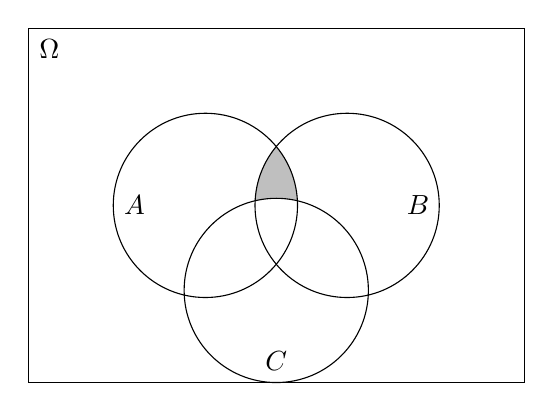
\begin{tikzpicture}[scale=0.9]
    % Durchschnitt von (A und  B) ohne C fuellen
    \begin{scope}
        \clip (2.5,2.5) circle (1.3cm);
        \clip (4.5,2.5) circle (1.3cm);
        \fill[gray, opacity=0.5] (2.5,2.5) circle (1.3cm);
        \fill[white] (3.5,1.3) circle (1.3cm);
    \end{scope}
    
    \draw (0,0) rectangle (7,5);
    \draw (2.5,2.5) circle (1.3cm);
    \draw (4.5,2.5) circle (1.3cm);
    \draw (3.5,1.3) circle (1.3cm);
    \node at (1.5,2.5) {$A$};
    \node at (5.5,2.5) {$B$};
    \node at (3.5,0.3) {$C$};
    \node at (0.3,4.7) {$\Omega$};
\end{tikzpicture}
\end{lstlisting}

\begin{ausgabe}
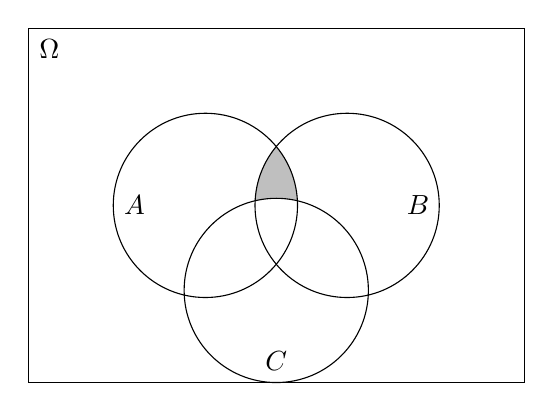
\begin{tikzpicture}[scale=0.9]
    \begin{scope}
        \clip (2.5,2.5) circle (1.3cm);
        \clip (4.5,2.5) circle (1.3cm);
        \fill[gray, opacity=0.5] (2.5,2.5) circle (1.3cm);
        \fill[white] (3.5,1.3) circle (1.3cm);
    \end{scope}
    \draw (0,0) rectangle (7,5);
    \draw (2.5,2.5) circle (1.3cm);
    \draw (4.5,2.5) circle (1.3cm);
    \draw (3.5,1.3) circle (1.3cm);
    \node at (1.5,2.5) {$A$};
    \node at (5.5,2.5) {$B$};
    \node at (3.5,0.3) {$C$};
    \node at (0.3,4.7) {$\Omega$};
\end{tikzpicture}
\end{ausgabe}

\subsection{Die Vereinigung $A \cup B \cup C$ füllen}

\begin{lstlisting}[style=latex]
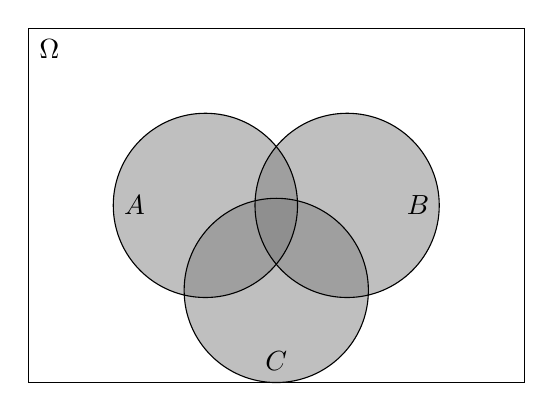
\begin{tikzpicture}[scale=0.9]
    % Vereinigung von A und B und C fuellen
    \begin{scope}
        \fill[gray, opacity=0.5] (2.5,2.5) circle (1.3cm);
        \fill[gray, opacity=0.5] (4.5,2.5) circle (1.3cm);
        \fill[gray, opacity=0.5] (3.5,1.3) circle (1.3cm);
    \end{scope}
    
    \draw (0,0) rectangle (7,5);
    \draw (2.5,2.5) circle (1.3cm);
    \draw (4.5,2.5) circle (1.3cm);
    \draw (3.5,1.3) circle (1.3cm);
    \node at (1.5,2.5) {$A$};
    \node at (5.5,2.5) {$B$};
    \node at (3.5,0.3) {$C$};
    \node at (0.3,4.7) {$\Omega$};
\end{tikzpicture}
\end{lstlisting}

\begin{ausgabe}
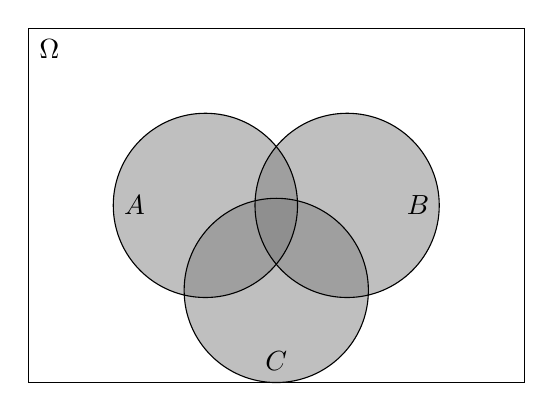
\begin{tikzpicture}[scale=0.9]
    \begin{scope}
        \fill[gray, opacity=0.5] (2.5,2.5) circle (1.3cm);
        \fill[gray, opacity=0.5] (4.5,2.5) circle (1.3cm);
        \fill[gray, opacity=0.5] (3.5,1.3) circle (1.3cm);
    \end{scope}
    \draw (0,0) rectangle (7,5);
    \draw (2.5,2.5) circle (1.3cm);
    \draw (4.5,2.5) circle (1.3cm);
    \draw (3.5,1.3) circle (1.3cm);
    \node at (1.5,2.5) {$A$};
    \node at (5.5,2.5) {$B$};
    \node at (3.5,0.3) {$C$};
    \node at (0.3,4.7) {$\Omega$};
\end{tikzpicture}
\end{ausgabe}

\subsection{Nur $A$ ohne Überschneidungen füllen: $A \setminus (B \cup C)$}

Dieser Bereich zeigt nur die Elemente, die ausschließlich in $A$ liegen:

\begin{lstlisting}[style=latex]
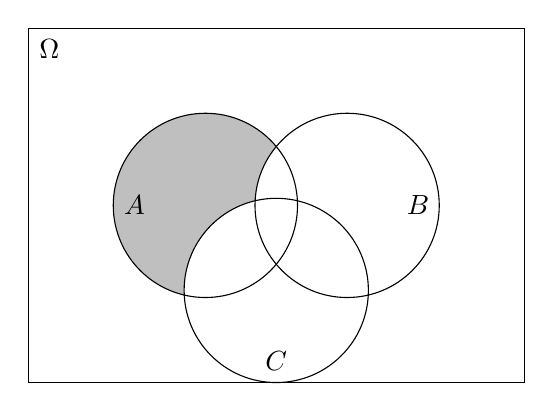
\begin{tikzpicture}[scale=0.9]
    % Nur A ohne Ueberschneidungen: A ohne (B vereinigt C)
    \begin{scope}
        \clip (2.5,2.5) circle (1.3cm);
        \fill[gray, opacity=0.5] (2.5,2.5) circle (1.3cm);
        \fill[white] (4.5,2.5) circle (1.3cm);
        \fill[white] (3.5,1.3) circle (1.3cm);
    \end{scope}
    
    \draw (0,0) rectangle (7,5);
    \draw (2.5,2.5) circle (1.3cm);
    \draw (4.5,2.5) circle (1.3cm);
    \draw (3.5,1.3) circle (1.3cm);
    \node at (1.5,2.5) {$A$};
    \node at (5.5,2.5) {$B$};
    \node at (3.5,0.3) {$C$};
    \node at (0.3,4.7) {$\Omega$};
\end{tikzpicture}
\end{lstlisting}

\begin{ausgabe}
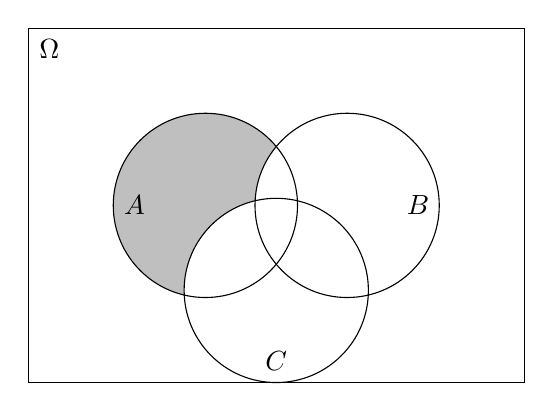
\begin{tikzpicture}[scale=0.9]
    \begin{scope}
        \clip (2.5,2.5) circle (1.3cm);
        \fill[gray, opacity=0.5] (2.5,2.5) circle (1.3cm);
        \fill[white] (4.5,2.5) circle (1.3cm);
        \fill[white] (3.5,1.3) circle (1.3cm);
    \end{scope}
    \draw (0,0) rectangle (7,5);
    \draw (2.5,2.5) circle (1.3cm);
    \draw (4.5,2.5) circle (1.3cm);
    \draw (3.5,1.3) circle (1.3cm);
    \node at (1.5,2.5) {$A$};
    \node at (5.5,2.5) {$B$};
    \node at (3.5,0.3) {$C$};
    \node at (0.3,4.7) {$\Omega$};
\end{tikzpicture}
\end{ausgabe}

\section{Verwendung von Mustern mit der \texttt{patterns}-Bibliothek}

Neben einfarbigen Füllungen können auch Muster verwendet werden, um verschiedene Mengenbereiche zu unterscheiden:

\begin{lstlisting}[style=latex]
\begin{tikzpicture}[scale=0.9]
    % Menge A mit horizontalen Linien fuellen
    \begin{scope}
        \clip (2.5,2.5) circle (1.3cm);
        \fill[pattern=horizontal lines, pattern color=gray] (2.5,2.5) circle (1.3cm);
        \fill[white] (4.5,2.5) circle (1.3cm);
        \fill[white] (3.5,1.3) circle (1.3cm);
    \end{scope}
    
    % Menge B mit vertikalen Linien fuellen
    \begin{scope}
        \clip (4.5,2.5) circle (1.3cm);
        \fill[pattern=vertical lines, pattern color=gray] (4.5,2.5) circle (1.3cm);
        \fill[white] (2.5,2.5) circle (1.3cm);
        \fill[white] (3.5,1.3) circle (1.3cm);
    \end{scope}
    
    \draw (0,0) rectangle (7,5);
    \draw (2.5,2.5) circle (1.3cm);
    \draw (4.5,2.5) circle (1.3cm);
    \draw (3.5,1.3) circle (1.3cm);
    \node at (1.5,2.5) {$A$};
    \node at (5.5,2.5) {$B$};
    \node at (3.5,0.3) {$C$};
    \node at (0.3,4.7) {$\Omega$};
\end{tikzpicture}
\end{lstlisting}

\begin{ausgabe}
\begin{tikzpicture}[scale=0.9]
    \begin{scope}
        \clip (2.5,2.5) circle (1.3cm);
        \fill[pattern=horizontal lines, pattern color=gray] (2.5,2.5) circle (1.3cm);
        \fill[white] (4.5,2.5) circle (1.3cm);
        \fill[white] (3.5,1.3) circle (1.3cm);
    \end{scope}
    \begin{scope}
        \clip (4.5,2.5) circle (1.3cm);
        \fill[pattern=vertical lines, pattern color=gray] (4.5,2.5) circle (1.3cm);
        \fill[white] (2.5,2.5) circle (1.3cm);
        \fill[white] (3.5,1.3) circle (1.3cm);
    \end{scope}
    \draw (0,0) rectangle (7,5);
    \draw (2.5,2.5) circle (1.3cm);
    \draw (4.5,2.5) circle (1.3cm);
    \draw (3.5,1.3) circle (1.3cm);
    \node at (1.5,2.5) {$A$};
    \node at (5.5,2.5) {$B$};
    \node at (3.5,0.3) {$C$};
    \node at (0.3,4.7) {$\Omega$};
\end{tikzpicture}
\end{ausgabe}

Verfügbare Muster umfassen unter anderem:
\begin{itemize}
\item \texttt{horizontal lines} -- horizontale Linien
\item \texttt{vertical lines} -- vertikale Linien
\item \texttt{north east lines} -- diagonale Linien von links unten nach rechts oben
\item \texttt{north west lines} -- diagonale Linien von rechts unten nach links oben
\item \texttt{dots} -- Punktmuster
\item \texttt{crosshatch} -- gekreuzte Linien
\end{itemize}

\section{Zusammenfassung}

Die Darstellung von Venn-Diagrammen mit TikZ basiert auf der geschickten Kombination von \texttt{scope}-Umgebungen, \texttt{clip}-Befehlen und Fülloperationen. Die wichtigsten Techniken sind:

\begin{itemize}
\item Verwendung von \texttt{scope} zur Begrenzung der Wirkung von \texttt{clip}-Befehlen
\item Clipping auf Kreise oder andere Formen, um Schnittbereiche zu isolieren
\item Weißes Füllen, um Bereiche auszusparen
\item Transparenz mit \texttt{opacity} für überlappende Bereiche
\item Muster aus der \texttt{patterns}-Bibliothek für abwechslungsreiche Darstellungen
\end{itemize}

Mit diesen Grundlagen können Sie beliebige Mengenoperationen visualisieren und Ihren Schülerinnen und Schülern die Konzepte der Mengenlehre anschaulich vermitteln. Die vorgestellten Techniken lassen sich auf komplexere Situationen mit mehr als drei Mengen erweitern, wobei die grundlegende Vorgehensweise dieselbe bleibt.

\end{document}